\documentclass[a4paper, 12pt]{article}
\usepackage{amsmath}
\usepackage{listings}
\usepackage{pgfplots}
\usepackage{bookmark}
\usepackage[T1]{fontenc}
\usepackage[utf8]{inputenc}
\usepackage[portuguese]{babel}
\usepackage{booktabs}
\usepackage{float}

\usepackage[margin=1in]{geometry}

\usepackage{hyperref}
\hypersetup{
    colorlinks,
    citecolor=black,
    filecolor=black,
    linkcolor=black,
    urlcolor=black
}

\newtheorem{definition}{Definição}[section]
\newtheorem{remark}{Observação}

\renewcommand{\lstlistingname}{Algoritmo}% Listing -> Algoritmo

\title{Estruturas de Dados e Algoritmos\\ \Large{Frequência II}}
\author{Carlos Menezes}
\date{\today}

\begin{document}

\maketitle

\newpage

\tableofcontents

\newpage

\section{Análise de Algoritmos}

\begin{definition}[Algoritmo]
    Sequência finita de ações executáveis que visam obter uma solução para um determinado tipo de problema.
\end{definition}

\begin{remark}
    Dois algoritmos que resolvem o mesmo problema podem ter eficiências diferentes. Um algoritmo rápido permite resolver um problema numa máquina lenta.
\end{remark}

Existem formas de avaliar as exigências de um algoritmo:
\begin{itemize}
    \item Empiricamente: observando a execução do programa;
    \item Experimentalmente: modelo simplificado do problema, estimando o comportamento futuro;
    \item Analiticamente: demonstrando a existência de uma função matemática que calcule as exigências do programa em relação aos parâmetros do problema.
\end{itemize}

\subsection{Crescimento}

\begin{remark}
    O tempo de execução geralmente dependente de um único parâmetro $N$: medida abstrata do tamanho do problema a considerar, usualmente relacionada com a quantidade de dados a processar.
\end{remark}

\newpage

\subsection{Notação Assimptótica}

\begin{remark}
    A análise do tempo de execução de um algoritmo só é útil para valores de $N$ elevados. É utilizado o \textbf{pior-case} como valor para complexidade, pois:\end{remark}

    \begin{itemize}
        \item representa um limite superior no tempo de execução;
        \item o valor médio é muitas vezes próximo do pior-caso.
    \end{itemize}

\begin{definition}[Notação Assimptótica]
    A notação assimptótica permite estabelecer taxas de crescimento dos tempos de execução dos algoritmos em função dos tamanhos das entradas. A complexidade assimptótica é expressa através da ordem de magnitude usando a notação \emph{big O}, $\mathbf{O}$.
\end{definition}

\begin{definition}[Ordem de Magnitude]
    A ordem de magnitude de uma função é igual à ordem do seu termo que cresce mais rapidamente.
\end{definition}

\paragraph{Exemplo}
    $$
        f(n)=n+n^2+1
    $$

    A ordem de magnitude de $f(n)$ é $\mathbf{O(n^2)}$.

\begin{remark}[Classes de complexidade comuns]\end{remark}
    \begin{itemize}
        \item Constante, $\mathbf{O(1)}$
        \begin{itemize}
            \item o número de instruções de um programa for executado um número limitado/constante de vezes            
        \end{itemize}
        \item Logarítmica, $\mathbf{O(\log(n))}$
        \begin{itemize}
            \item um problema é resolvido através da resolução de um conjunto de subproblemas
        \end{itemize}
        \item Polinomial, $\mathbf{O(n^p), p \geq 1}$
        \begin{itemize}
            \item Linear, $\mathbf{O(n)}$
            \begin{itemize}
                \item quando existe algum processamento para cada elemento de entrada
            \end{itemize}
            \item Pseudo-linear, $\mathbf{O(n\log(n))}$
            \begin{itemize}
                \item Quando um problema é resolvido através da resolução de um conjunto de subproblemas, e combinando posteriormente as suas soluções
            \end{itemize}
            \item Quadrática, $\mathbf{O(n^2)}$
            \begin{itemize}
                \item quando a dimensão da entrada duplica, o tempo aumenta 4x
            \end{itemize}
            \item Cúbica, $\mathbf{O(n^3)}$
            \begin{itemize}
                \item quando a dimensão de entrada duplica o tempo aumenta 8x
            \end{itemize}
        \end{itemize}
        \item Exponencial, $\mathbf{O(p^n)}, n \geq 1$
        \begin{itemize}
            \item quando a dimensão de entrada duplica o tempo aumenta para o quadrado
        \end{itemize}
        \item Factorial, $\mathbf{O(n!)}$
    \end{itemize}


\begin{remark}[Garantias, previsões e limitações]
    O tempo de execução dos algoritmos depende criticamente dos dados. O objeto da análise de complexidade é inferir o máximo de informação assumindo o mínimo possível.
\end{remark}

\begin{remark}[Estudo do pior caso]\end{remark}
    O estudo do pior caso permite obter garantias máximas.
    \begin{itemize}
        \item se o resultado no pior caso é aceitável, então a situação é favorável;
        \item se o resultado no pior caso for mau, pode ser problemático;
    \end{itemize}


\begin{remark}[Estudo do melhor caso]\end{remark}
    Por vezes é relevante obter também limites inferiores. Esta análise pode dar indicações preciosas sobre como e onde melhorar o
    desempenho de um algoritmo. Se os limites inferiores e superiores forem próximos, é conveniente tentar otimizar a implementação.
    \begin{itemize}
        \item se o resultado no pior caso é aceitável, então a situação é favorável;
        \item se o resultado no pior caso for mau, pode ser problemático;
    \end{itemize}

\newpage

\section{Algoritmos de Ordenação}

\subsection{Insertion Sort}

\begin{remark}[Caraterísticas]\end{remark}
    Este algoritmo começa tratando  a primeiro entrada \texttt{A[0]} como um array já ordenado e, em seguida, verifica a segunda entrada \texttt{A[1]} e compara-a com
a primeiro. Se eles estiverem na ordem errada, é efetuada a troca. Com isto, temos \texttt{A[0]} e \texttt{A[1]} ordenados.
Em seguida, repete o processo para terceira entrada, posicionando-a no lugar certo, deixando \texttt{A[0]}, \texttt{A[1]} e \texttt{A[2]} ordenados. De forma mais geral, no início do $i$-ésimo ciclo, o insertion sort tem o
entradas \texttt{A[0],...,\texttt{A[i-1]}} ordenadas e inserte \texttt{A[i]}, ordenando as entradas \texttt{A[0], ..., \texttt{A[i]}}.
    \begin{itemize}
        \item simples implementação;
        \item requer uma quantidade constante de memória adicional;
        \item útil para pequenas entradas;
        \item muitas trocas e menos comparações.
        \item \textbf{Best Case}: $O(n)$
        \item \textbf{Average Case}: $O()\frac{n^2}{4})$
        \item \textbf{Worst Case}: $O(n^2)$
    \end{itemize}


\begin{center}
    \begin{lstlisting}[frame=single, language=c, caption=Algoritmo Insertion Sort, captionpos=b]
for ( i = 1 ; i < n ; i++ ) {
    for( j = i ; j > 0 ; j-- )
        if ( a[j] < a[j-1] )
            swap a[j] and a[j-1]
        else break
}            
    \end{lstlisting}

    \begin{figure}[H]
        \centering
        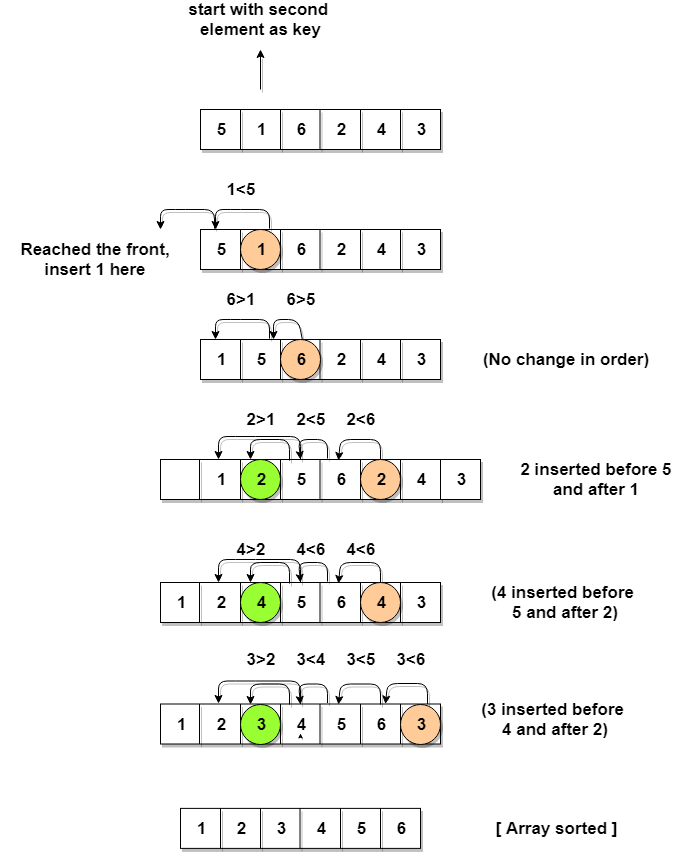
\includegraphics[width=0.5\textwidth]{fig/ao/is.png}
        \caption{Visualização do algoritmo Insertion Sort.}
    \end{figure}
\end{center}

\subsection{Selection Sort}
\begin{remark}[Caraterísticas]
    Este algoritmo encontra o menor item o coloca-o em \texttt{A[0]}, trocando-o por qualquer item que já esteja nessa posição. De seguida, encontra o segundo menor item e troca-o pelo item em \texttt{A[1]}. Este processo é repetido até que todo o array esteja ordenado.
    De modo mais geral, no $i$-ésimo ciclo, o Selection Sort encontra o $i$-ésimo item menor e troca-o com o item em $A[i-1]$.\end{remark}
    \begin{itemize}
        \item simples implementação;
        \item requer uma quantidade constante de memória adicional;
        \item útil para pequenas entradas;
        \item \textbf{Best Case}: $O(n^2)$
        \item \textbf{Average Case}: $O(n^2)$
        \item \textbf{Worst Case}: $O(n^2)$
    \end{itemize}


\begin{center}
    \begin{lstlisting}[frame=single, language=c, caption=Algoritmo Selection Sort, captionpos=b]
for ( i = 0 ; i < n-1 ; i++ ) {
    k = i
    for ( j = i+1 ; j < n ; j++ )
        if ( a[j] < a[k] )
            k = j
    swap a[i] and a[k]
}          
    \end{lstlisting}
    
    \begin{figure}[H]
        \centering
        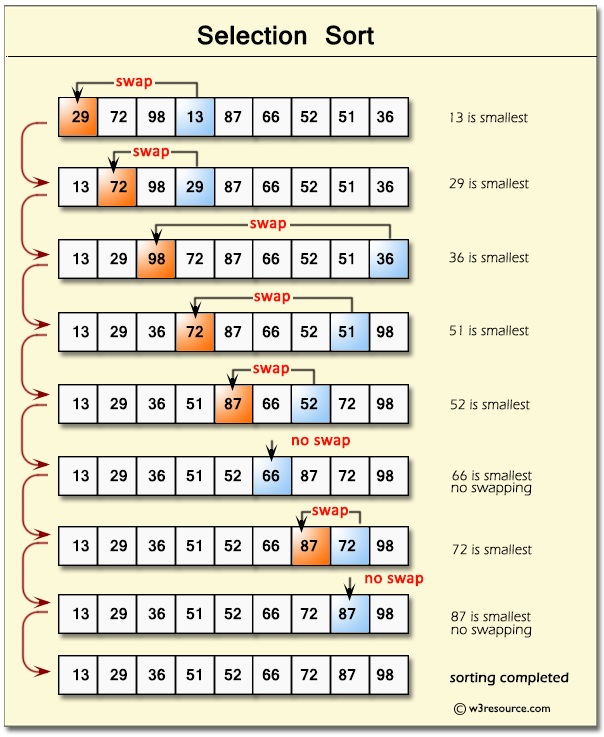
\includegraphics[width=0.5\textwidth]{fig/ao/ss.png}
        \caption{Visualização do algoritmo Selection Sort.}
    \end{figure}
\end{center}

\subsection{Bubble Sort}
\begin{remark}[Caraterísticas]
    Este algoritmo começa comparando \texttt{A[n-1]} com \texttt{A[n-2]} e troca-os se estiverem na ordem errada. Em seguida, compara \texttt{A[n-2]} e \texttt{A[n-3]} e troca-os, se necessário, e assim por diante. Quando atinge \texttt{A[0]}, a menor entrada estará no local correto. Em seguida, começa de trás novamente, comparando pares de "vizinhos" a partir de \texttt{A[1]}. De modo mais geral, no $i$-ésimo ciclo, o Bubble Sort compara os vizinhos desde trás, trocandoo-os quando necessário. O item com o índice mais baixo que é comprado com o seu vizinho da direita é \texttt{A[i-1]}. Após o $i$-ésimo ciclo, as entradas \texttt{A[0],...,A[i-1]} estão na sua posição final.\end{remark}
    \begin{itemize}
        \item simples implementação;
        \item requer uma quantidade constante de memória adicional;
        \item \textbf{Best Case}: $O(n)$
        \item \textbf{Average Case}: $O(n^2)$
        \item \textbf{Worst Case}: $O(n^2)$
    \end{itemize}


\begin{center}
    \begin{lstlisting}[frame=single, language=c, caption=Algoritmo Bubble Sort, captionpos=b]
for ( i = 1 ; i < n ; i++ )
    for ( j = n-1 ; j >= i ; j-- )
        if ( a[j] < a[j-1] )
            swap a[j] and a[j-1]
    \end{lstlisting}
    
    \begin{figure}[H]
        \centering
        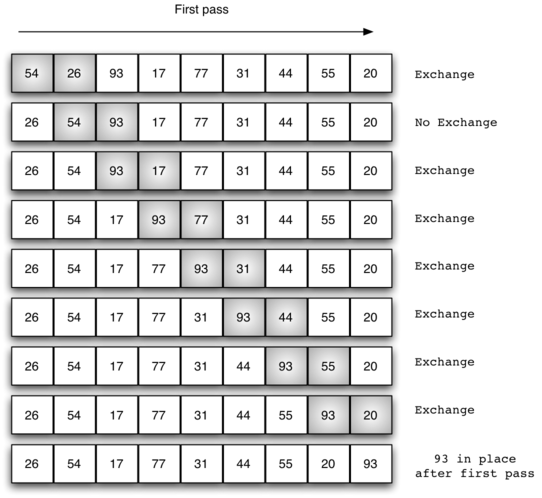
\includegraphics[width=0.5\textwidth]{fig/ao/bs.png}
        \caption{Visualização do algoritmo Bubble Sort.}
    \end{figure}
\end{center}

\subsection{Shell Sort}
\begin{remark}[Caraterísticas]
    Este algoritmo primeiro classifica os elementos distantes uns dos outros e reduz sucessivamente o intervalo entre os elementos a serem classificados. É uma versão generalizada do Insertion Sort. De modo geral, o algoritmo passa várias vezes pela lista dividindo o grupo maior em menores, onde é aplicado o Insertion Sort.\end{remark}
    \begin{itemize}
        \item \textbf{Best Case}: $O(n\log n)$
        \item \textbf{Average Case}: $O(n\log n)$
        \item \textbf{Worst Case}: $O(n^2)$
    \end{itemize}


\begin{center}
    \begin{lstlisting}[frame=single, language=c, caption=Algoritmo Shell Sort, captionpos=b]
for (int gap = n/2; gap > 0; gap /= 2)
{
    for (int i = gap; i < n; i += 1)
    {
        int temp = arr[i];
        int j;            
        for (j = i; j >= gap && arr[j - gap] > temp; j -= gap)
            arr[j] = arr[j - gap];
        arr[j] = temp;
    }
}
    \end{lstlisting}
    
    \begin{figure}[H]
        \centering
        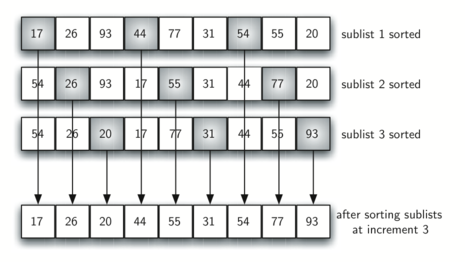
\includegraphics[width=0.8\textwidth]{fig/ao/shs.png}
        \caption{Visualização do algoritmo Shell Sort.}
    \end{figure}
\end{center}

\subsection{Merge Sort}
\begin{remark}[Caraterísticas]
    Este algoritmo utiliza a técnica divisão e conquista: a solução é encontrada à custa da mesma solução mas com argumentos estruturalmente mais simples.\end{remark}
    \begin{itemize}
        \item se o número de partes é $\leq$ 1, terminar;
        \item dividir o vetor em 2 partes;
        \item ordenar recursivamente as duas partes;
        \item fundir as metades ordenadas;
    \end{itemize}
    \begin{itemize}
        \item requer a utilização de um vetor adicional;
        \item \textbf{Best Case}: $O(n\log n)$
        \item \textbf{Average Case}: $O(n\log n)$
        \item \textbf{Worst Case}: $O(n\log n)$
    \end{itemize}


\begin{center}
    \begin{figure}[H]
        \centering
        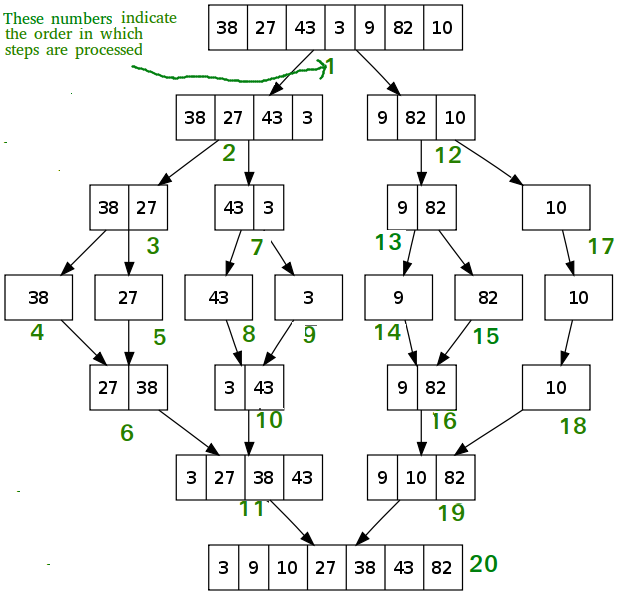
\includegraphics[width=0.8\textwidth]{fig/ao/ms.png}
        \caption{Visualização do algoritmo Merge Sort.}
    \end{figure}
\end{center}

\subsection{Quick Sort}
\begin{remark}[Caraterísticas]
    Este algoritmo utiliza a técnica divisão e conquista: a solução é encontrada à custa da mesma solução mas com argumentos estruturalmente mais simples.\end{remark}
    \begin{itemize}
        \item se o número de partes é $\leq$ 1, terminar;
        \item escolher um item arbitrário — \textbf{pivot} (e.g. o último ou o 1º);
        \item rearranjar os restantes elementos em dois grupos:
        \begin{itemize}
            \item elementos com menor valor do que o pivot à esquerda do pivot;
            \item elementos com maior valor do que o pivot à direita do pivot;
        \end{itemize}
        \item repetir processo anterior às listas esquerda e direita até chegar a listas com, no máximo, 1 elemento.
    \end{itemize}
    \begin{itemize}
        \item requer a utilização de um vetor adicional;
        \item \textbf{Best Case}: $O(n\log n)$
        \item \textbf{Average Case}: $O(n\log n)$
        \item \textbf{Worst Case}: $O(n^2)$
    \end{itemize}
\begin{center}
    \begin{figure}[H]
        \centering
        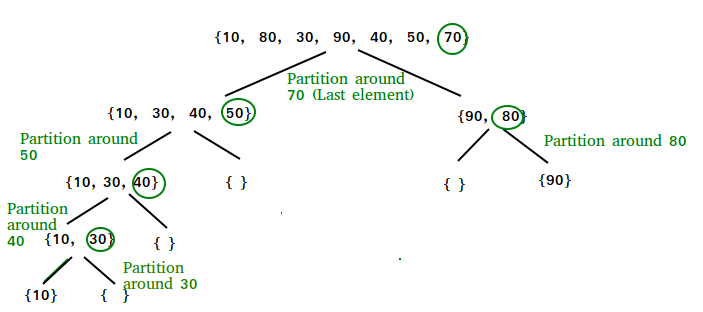
\includegraphics[width=0.8\textwidth]{fig/ao/qs.png}
        \caption{Visualização do algoritmo Quick Sort.}
    \end{figure}
\end{center}

\subsection{Sumário}

\begin{center}
    \begin{figure}[H]
        \centering
        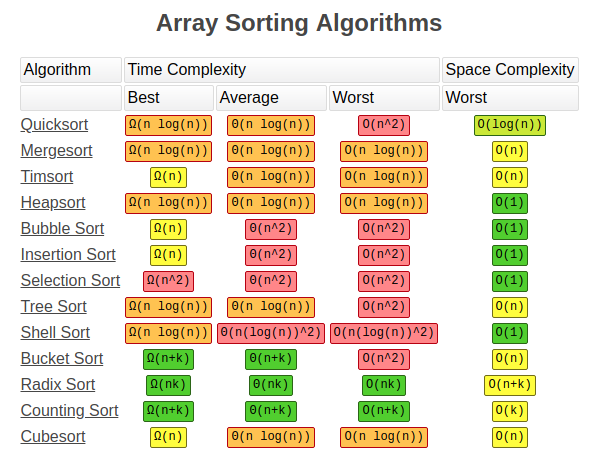
\includegraphics[width=0.8\textwidth]{fig/ao/sumario.png}
        \caption{Sumário de algoritmos de ordenação.}
    \end{figure}
\end{center}

\newpage

\section{Recursividade}

\begin{definition}[Recursividade.]
    A recursão é um método de resolver um problema em que a solução depende de soluções para instâncias menores do mesmo problema.
\end{definition}

\begin{remark}
    Um programa recursivo não se pode chamar a si próprio infinitas vezes, caso contrário nunca pararia. Deste modo, é essencial existir uma \textbf{condição de paragem}.\end{remark}
\begin{itemize}
    \item apesar das vantagens das implementações recursivas, é relativamente fácil escrever funções recursivas que são extremamente ineficientes.
    \item características básicas de um qualquer programa recursivo:
    \begin{itemize}
        \item chama-se a si próprio para valores menores do seu argumento;
        \item possui uma condição de paragem em que calcula o resultado diretamente.
    \end{itemize}
\end{itemize}


\begin{remark}[Divisão e Conquista.]\end{remark}
    Este problemas consistem em:
    \begin{itemize}
        \item divisão em partes de tamanhos variáveis;
        \item divisão em mais que duas partes;
        \item divisão em partes que se sobrepõem;
        \item realizar diversas quantidades de cálculos na componente não recursiva do algoritmo.
    \end{itemize}

    Geralmente, estes algoritmos realizam cálculos para:
    \begin{itemize}
        \item dividir a entrada em partes;
        \item combinar os resultados obtidos em cada parte;
        \item facilitar os cálculos entre as duas chamadas.
    \end{itemize}

\begin{remark}[Estratégias.]\end{remark}
    \begin{itemize}
        \item divisão e conquista:
        \begin{itemize}
            \item problema é partido em sub-problemas que se resolvem separadamente;
            \item solução obtida por combinações das soluções;
        \end{itemize}
        \item Programação dinâmica:
        \begin{itemize}
            \item  resolvem-se os problemas de pequena dimensão e guardam-se as soluções;
            \item solução de um problema é obtida combinando as de problemas de menor dimensão.
        \end{itemize}
    \end{itemize}

\newpage

\section{Árvores}

\begin{definition}[Árvore.]
    Uma árvore é um tipo de dados abstrato amplamente usado que simula uma estrutura de árvore hierárquica, com um valor raiz e subárvores de filhos com um nó pai, representados como um conjunto de nós vinculados.
\end{definition}

\begin{remark}[\emph{Nodes}]\end{remark}

    \begin{itemize}
        \item cada \emph{node} pode possuir um número variável de nós descendentes diretos;
        \item \emph{nodes} com o mesmo ascendente direto designam-se por \emph{siblings};
        \item um \emph{node} sem ascendente designa-se por \emph{root} (é único numa árvore).
    \end{itemize}
    \begin{center}
        \begin{figure}[H]
            \centering
            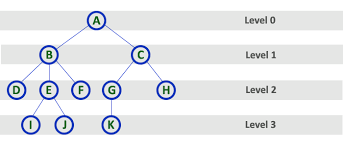
\includegraphics[width=0.5\textwidth]{fig/t/tlevels.png}
            \caption{Níveis de uma árvore.}
        \end{figure}
    \end{center}


\begin{remark}[Terminologia]\end{remark}
    \begin{itemize}
        \item \textbf{caminho}: sequência de \emph{nodes} desde a \emph{root} até a uma \emph{leaf};
        \begin{itemize}
            \item a \textbf{dimensão} de um caminho corresponde ao seu número de nós.
        \end{itemize}
        \item a \textbf{altura}/\textbf{profundidade} de uma árvore é a maior dimensão do maior caminho (número de níveis).
        \item \textbf{Grau} ou \textbf{aridade} de:
        \begin{itemize}
            \item um \emph{node}: número de \emph{children nodes};
            \item uma árvore: maior grau dos seus \emph{nodes}.
        \end{itemize}
        \item \textbf{subárvore} de um \emph{node} é a árvore com \emph{root} nesse \emph{node};
        \item \textbf{árvores degeneradas} são árvores de grau 1 (e.g. listas).
    \end{itemize}


\subsection{Árvores Binárias}
\begin{center}
    \begin{figure}[H]
        \centering
        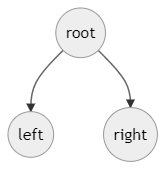
\includegraphics[width=0.2\textwidth]{fig/t/tb.png}
        \caption{Árvore binária.}
    \end{figure}
\end{center}
\begin{itemize}
    \item árvores de grau 2;
    \begin{itemize}
        \item cada \emph{node} pode ter até dois descendentes;
        \item contêm duas subárvores (que podem ser vazias);
        \item é usual considerar a notação infixa: $<A_1;x;A_2>$ (esquerda; \emph{node}; direita);
        \item \textbf{árvore estritamente binária}: todos os nós têm grau 0 ou 2;
        \item \textbf{árvore binária equilibrada}: a diferença entre as alturas das subárvores não é superior a 1 e todas as subárvores são equilibradas;
        \item uma árvore binária está \textbf{cheia} se:
        \begin{itemize}
            \item for vazia, ou;
            \item as subárvores tiverem a mesma altura e estiverem cheias (se $d$ é a altura da árvore, então esta é formada por $2^d-1$ \emph{nodes});
        \end{itemize}
        \item uma árvore binária de altura $h$ está completa se estiver cheia até ao nível $h-1$ e todos os nós do último nível estão o mais à esquerda possível.
        \begin{center}
            \begin{figure}[H]
                \centering
                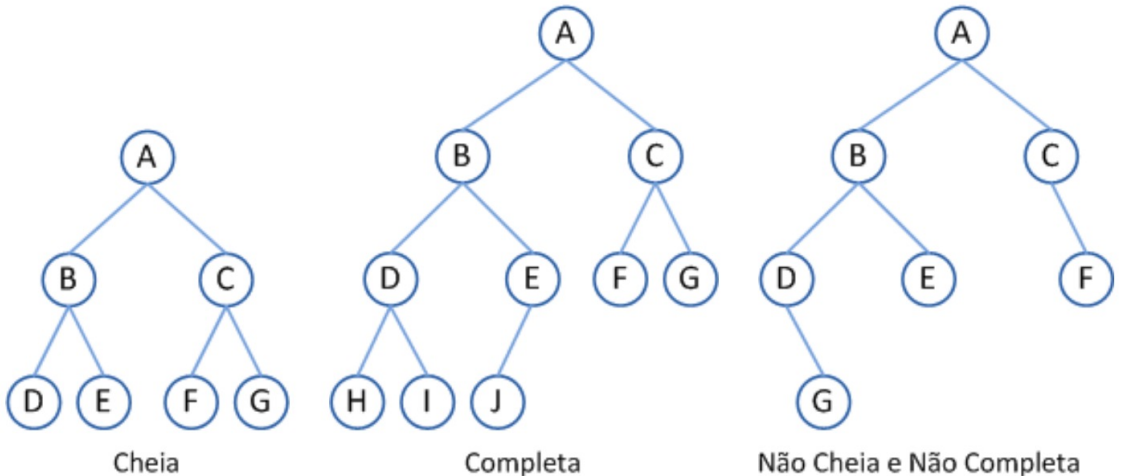
\includegraphics[width=0.5\textwidth]{fig/t/btcompletefull.png}
            \end{figure}
        \end{center}
    \end{itemize}
\end{itemize}

\begin{remark}[Pesquisa de um elemento]\end{remark}
\begin{itemize}
    \item realização de travessias em profundidade:
    \begin{itemize}
        \item prefixa;
        \item infixa;
        \item sufixa;
    \end{itemize}
    \item realização de travessias em largura.
\end{itemize}

\paragraph{Travessia Prefixa, \textbf{RLR}}
\begin{enumerate}
    \item visitar o \emph{root node};
    \item travessia prefixa da subárvore esquerda;
    \item travessia prefixa da subárvore direita;
\end{enumerate}

\paragraph{Travessia Infixa, \textbf{LRR}}
\begin{enumerate}
    \item travessia infixa da subárvore esquerda;
    \item visitar o \emph{root node};
    \item travessia infixa da subárvore direita;
\end{enumerate}

\paragraph{Travessia Sufixa, \textbf{LRR}}
\begin{enumerate}
    \item travessia sufixa da subárvore esquerda;
    \item travessia sufixa da subárvore direita;
    \item visitar o \emph{root node};
\end{enumerate}

\paragraph{Travessia em Largura}
\begin{enumerate}
    \item visitar o \emph{root node};
    \item visitar os \emph{nodes} de cada nível, da esquerda para a direita;
\end{enumerate}

\subsection{Árvores de Pesquisa Binária}
Numa árvore de pesquisa binária, os valores são inseridos após serem comparados com o valor raiz:
\begin{itemize}
    \item valores maiores à direita;
    \item valores menores à esquerda;
    \item utiliza-se a recursão para inserir novos valores;
    \item a inserção é feita nos \emph{leaf nodes}.
\end{itemize}

\begin{remark}[Remoção de Elementos]
    Existem dois métodos para a remoção de \emph{nodes}: por \textbf{fusão}; por \textbf{cópia}.
\end{remark}

\begin{remark}[Remoção por cópia.]
\end{remark}
\begin{figure}[H]
    \centering
    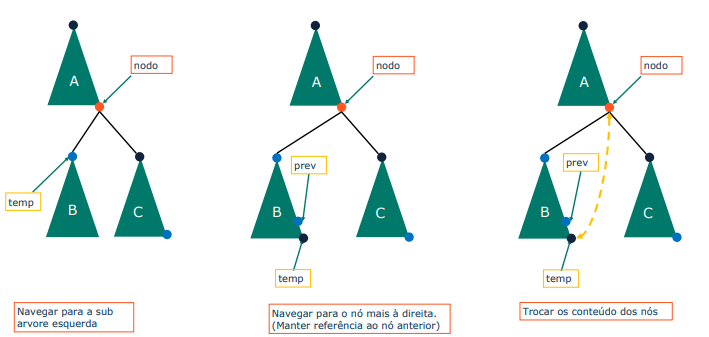
\includegraphics[width=0.8\textwidth]{fig/t/bstRemoveCopy.png}
    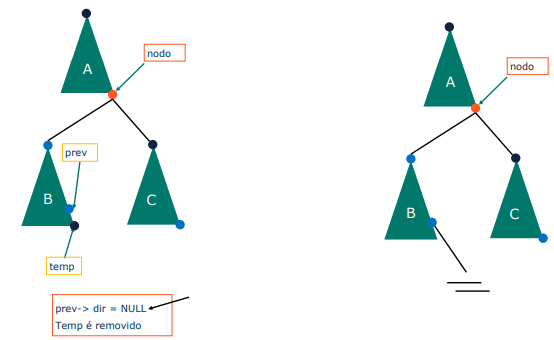
\includegraphics[width=0.8\textwidth]{fig/t/bstRemoveCopy2.png}
    \caption{Remoção de \emph{node} por cópia.}
\end{figure}

\begin{remark}[Remoção por fusão.]
\end{remark}
\begin{figure}[H]
    \centering
    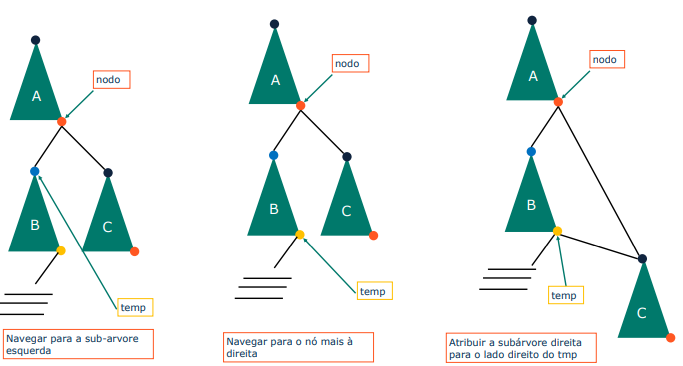
\includegraphics[width=0.8\textwidth]{fig/t/bstRemoveFusion.png}
    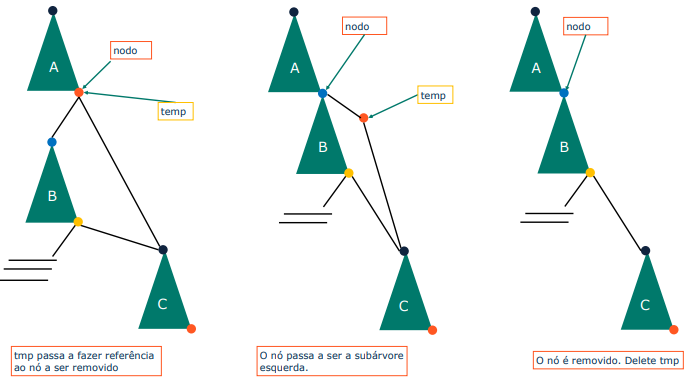
\includegraphics[width=0.8\textwidth]{fig/t/bstRemoveFusion2.png}
    \caption{Remoção de \emph{node} por fusão.}
\end{figure}

\subsection{Árvores AVL}
As árvores AVL são BSTs com equilíbrio de altura. A árvore AVL verifica a altura das subárvores esquerda e direita e garante que a diferença não seja maior do que 1. Essa diferença é chamada de \textbf{Fator de Balanceamento}, $FB$.

A figura abaixo exemplifica uma árvore balanceada e duas não balanceadas:

\begin{figure}[H]
    \centering
    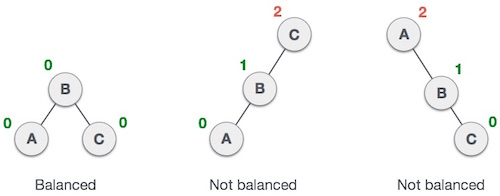
\includegraphics[width=0.8\textwidth]{fig/t/unbalanced_avl_trees.jpg}
    \caption{Árvores (não) balanceadas.}
\end{figure}

Na segunda árvore, a subárvore esquerda de C tem altura 2 e a subárvore direita tem altura 0, então a diferença é 2. Na terceira árvore, a subárvore direita de A tem altura 2 e a esquerda está em falta, pelo que a sua altura é 0; a diferença é 2 novamente. A árvore AVL permite que a diferença (fator de equilíbrio) seja apenas 1.

\begin{equation}
    FB=altura(raiz\_esquerda)-altura(raiz\_direita)
\end{equation}

\subsubsection{Rotações}
De modo a se equilibrar, uma árvore AVL pode realizar os seguintes quatro tipos de rotações:

\begin{itemize}
    \item Rotação à Esquerda (L)
    \item Rotação à Direita (R)
    \item Rotação Esquerda-Direita (LR)
    \item Rotação Direita-Esquerda (RL)
\end{itemize}

As duas primeiras rotações são rotações simples e as duas rotações seguintes são rotações duplas.

\begin{remark}[Rotação à Esquerda, L]\end{remark}
\begin{figure}[H]
    \centering
    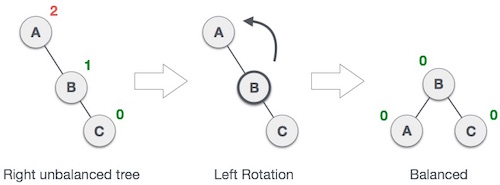
\includegraphics[width=0.5\textwidth]{fig/t/avl_left_rotation.jpg}
    \caption{Rotação L.}
\end{figure}

\begin{remark}[Rotação à Direita, R]\end{remark}
\begin{figure}[H]
    \centering
    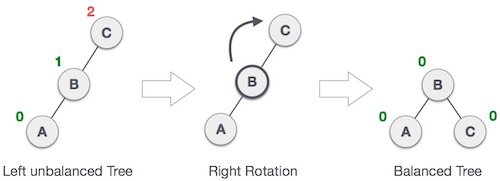
\includegraphics[width=0.5\textwidth]{fig/t/avl_right_rotation.jpg}
    \caption{Rotação R.}
\end{figure}

\begin{remark}[Rotação à Esquerda-Direita, LR]\end{remark}
\begin{figure}[H]
    \centering
    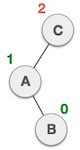
\includegraphics[width=2cm]{fig/t/right_subtree_of_left_subtree.jpg}
    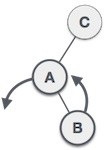
\includegraphics[width=2cm]{fig/t/subtree_left_rotation.jpg}
    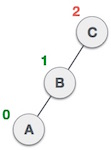
\includegraphics[width=2cm]{fig/t/left_unbalanced_tree.jpg}
    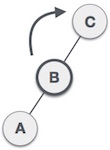
\includegraphics[width=2cm]{fig/t/right_rotation.jpg}
    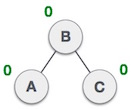
\includegraphics[width=2cm]{fig/t/balanced_avl_tree.jpg}
    \caption{Rotação LR.}
\end{figure}

\begin{remark}[Rotação à Direita-Esquerda, RL]\end{remark}
\begin{figure}[H]
    \centering
    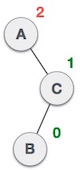
\includegraphics[width=2cm]{fig/t/left_subtree_of_right_subtree.jpg}
    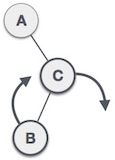
\includegraphics[width=2cm]{fig/t/subtree_right_rotation.jpg}
    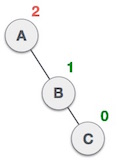
\includegraphics[width=2cm]{fig/t/right_unbalanced_tree.jpg}
    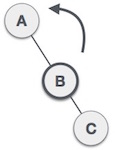
\includegraphics[width=2cm]{fig/t/left_rotation.jpg}
    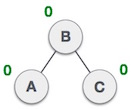
\includegraphics[width=2cm]{fig/t/balanced_avl_tree (1).jpg}
    \caption{Rotação RL.}
\end{figure}

\newpage

\section{Heap}

Um Heap é um caso especial de estrutura de dados de árvore binária balanceada, em que a chave do \emph{root node} é comparada com seus filhos e organizada de acordo com o tipo de heap.

Geralmente, as Heaps podem ser de dois tipos:

\begin{enumerate}
    \item \textbf{Max-Heap}: a chave presente no \emph{root} node deve ser a chave com maior valor entre os seus filhos. A mesma propriedade deve ser recursivamente verdadeira para todas as subárvores.
    \item \textbf{Min-Heap}: a chave presente no \emph{root} node deve ser a chave com menor valor entre os seus filhos. A mesma propriedade deve ser recursivamente verdadeira para todas as subárvores.
\end{enumerate}

\begin{figure}[H]
    \centering
    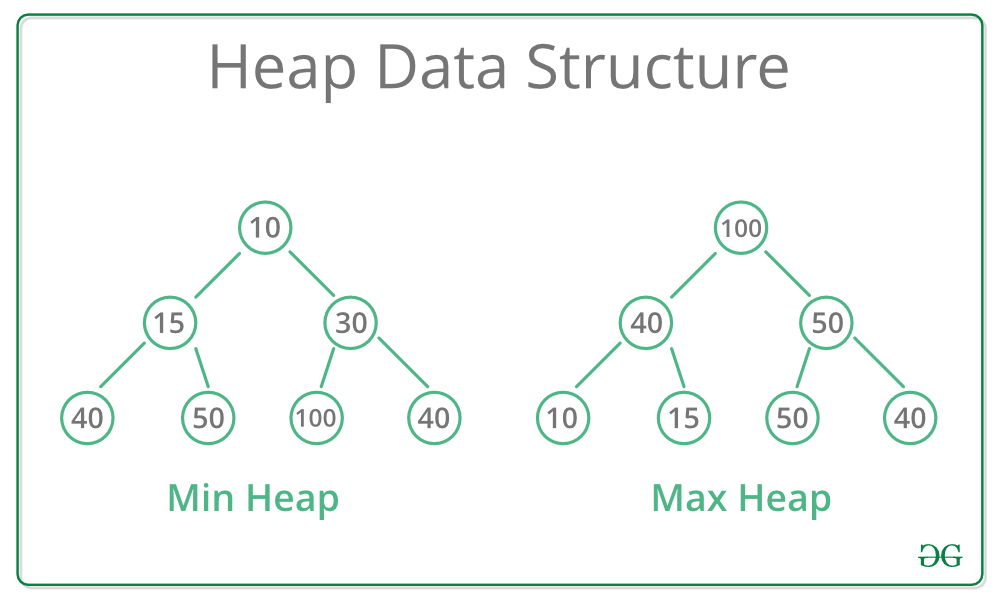
\includegraphics[width=0.6\textwidth]{fig/heaps/MinHeapAndMaxHeap.png}
    \caption{Tipos de \emph{heap}.}
\end{figure}

\begin{remark}[Representação vetorial.]
    A representação vetorial de um \emph{heap} é feita colocando a ordem de visita dos seus elementos numa travessia em profundidade.
\end{remark}

\subsection{Max-Heap}
\subsubsection{Inserção}
\begin{enumerate}
    \item criar um novo \emph{node} no fim do \emph{heap};
    \item atribuir novo valor ao \emph{node};
    \item comparar o valor deste \emph{node} filho com o seu pai;
    \begin{enumerate}
        \item se o valor do pai for inferior ao do filho, trocam (troca pelo maior);
    \end{enumerate}
\end{enumerate}

\textbf{Contrução de um max-heap}: \url{https://www.tutorialspoint.com/data_structures_algorithms/images/max_heap_animation.gif}

\subsubsection{Remoção}
\begin{enumerate}
    \item remover \emph{root node};
    \item mover o último elemento do último nível para a raiz;
    \item comparar o valor dos descendentes com este \emph{node};
    \begin{enumerate}
        \item se o valor do pai for inferior ao do filho, trocam (troca pelo maior);
    \end{enumerate}
\end{enumerate}

\textbf{Remoção num max-heap}: \url{https://www.tutorialspoint.com/data_structures_algorithms/images/max_heap_deletion_animation.gif}

\subsection{Heapsort}
O algoritmo \emph{Heapsort} tem duas partes principais (que serão divididas mais adiante): construir um max-heap e, em seguida, ordená-lo. O max-heap é construído conforme descrito na seção acima. Em seguida, o \emph{Heapsort} produz um array ordenado removendo repetidamente o maior elemento do heap (que é a raiz do heap) e, em seguida, inserindo-o no array. O heap é atualizado após cada remoção. Depois de todos os elementos serem removidos do heap, o resultado é um array ordenada.

\begin{enumerate}
    \item construit um max-heap;
    \item depois do heap estar criado, repetidamente eliminar o elemento raiz do heap deslocando-o para o final do array e, a seguir, armazenar a estrutura do heap com os elementos restantes.
\end{enumerate}

\textbf{Heapsort:} \url{https://www.interviewbit.com/tutorial/heap-sort-algorithm/} 

\newpage

\section{Hash Tables}
Uma Hash Table é uma estrutura de dados que armazena dados de forma associativa. Numa tabela hash, os dados são armazenados num formato de array, em que cada valor de dados tem seu próprio valor de índice exclusivo. O acesso aos dados torna-se muito rápido se conhecermos o índice dos dados desejados. Assim, torna-se uma estrutura de dados em que as operações de inserção e busca são muito rápidas, independentemente do tamanho dos dados.

\subsection{Hashing}
\begin{figure}[H]
    \centering
    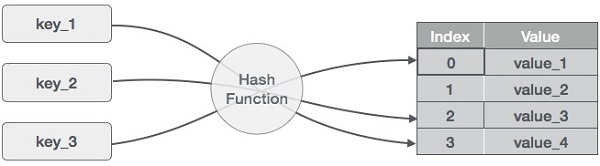
\includegraphics[width=0.6\textwidth]{fig/hash/hash_function.jpg}
    \caption{Função de \emph{hash}.}
\end{figure}

\subsubsection{Colisões}
\begin{remark}[Endereçamento Fechado]
Elementos cuja chave devolve o mesmo valor de dispersão são armazenados numa lista.

\begin{figure}[H]
    \centering
    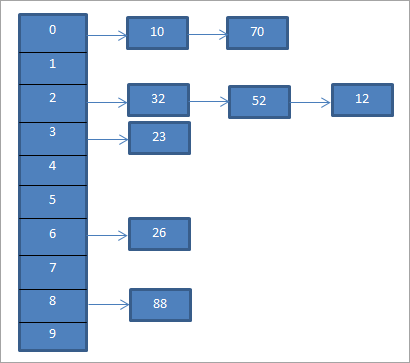
\includegraphics[width=0.6\textwidth]{fig/hash/1_m8pm0demNgJnaeN7W9JWew.png}
    \caption{Endereçamento fechado.}
\end{figure}
\end{remark}

\begin{remark}[Endereçamento Aberto]
No método de endereçamento aberto os registros em conflito são armazenados dentro da própria tabela de dispersão. A resolução das colisões é realizada através de buscas padronizadas dentro da própria tabela. A forma mais simples de fazer a busca é procurar linearmente na tabela até encontrar um registo vazio.
    
Neste caso, é necessária outra função que permita encontrar posições alternativas — \textbf{linear probing}:

\begin{equation}
    P=(1+P) \mod{table\_size}
\end{equation}
\end{remark}

\begin{figure}[H]
    \centering
    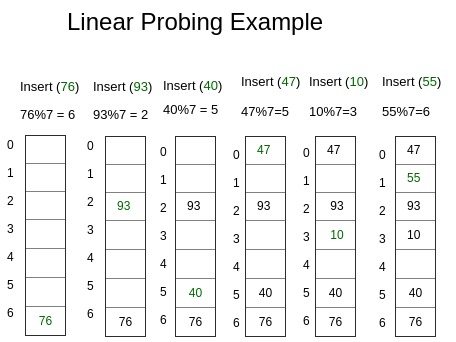
\includegraphics[width=0.6\textwidth]{fig/hash/Linear-Probing-1-1.jpg}
    \caption{\emph{Linear probing}.}
\end{figure}

\begin{remark}[Linear Probing c/ Double Hashing]
Incrementar a equação acima com um valor que depende da chave.
\end{remark}

\begin{equation}
    P=(P+INCREMENTO(CHAVE)) \mod table\_size
\end{equation}
\end{document}